\textbf{COLUNI 2022 -- Questão 24}\par\medskip A figura abaixo mostra a vista aérea da trajetória de um carro viajando em uma estrada plana. Ao chegar no ponto P, o carro entra em uma área grande, coberta de óleo. Isso reduz o atrito entre os pneus e o solo, nessa região, a zero. Assinale a alternativa cuja trajetória pontilhada corresponde CORRETAMENTE àquela seguida pelo veículo a partir do ponto P:

% COLUNI-AUTO-FIGURES-BEGIN
\begin{figure}[htbp]
\centering
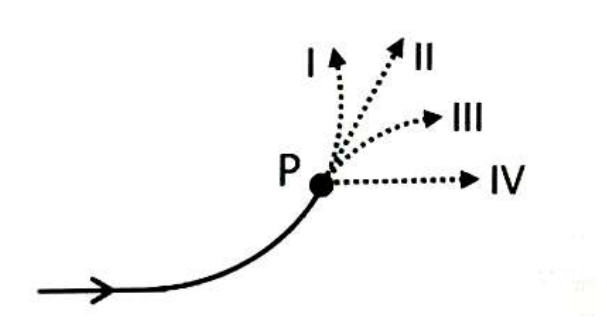
\includegraphics[width=0.95\linewidth]{static/simulados/coluni/figuras/2022/questao-24/figura-1.png}
\end{figure}
% COLUNI-AUTO-FIGURES-END

\par

a) I\par
b) II\par
c) III\par
d) IV



